\documentclass[12pt]{article}
\usepackage{setspace}
\singlespacing

\usepackage{amsmath}
\usepackage[margin = 1in]{geometry}
\usepackage{graphicx}
\usepackage{booktabs}
\usepackage{natbib}
\usepackage[colorlinks=true, citecolor=blue]{hyperref}
\usepackage{indentfirst}

\title{Predicting Diabetes Based on Various Factors Using Decision Tree Analysis}
\author{Ashley Merritt\\
    Department of Statistics\\
    University of Connecticut
    }

\begin{document}
\maketitle

\begin{abstract}
Each year, many patients learn that they have diabetes and are left wondering what could have done to prevent the diagnosis. This
paper uses decision tree modeling to investigate which predictors of the Healthcare Diabetes dataset from kaggle are important in predicting 
an outcome of diabetes. In this study, after exploratory data analysis, the data was split into a training and testing set
that will be used to build a decision tree. The performance was evaluated using standard classification metrics, including accuracy, precision, 
recall, and F1 score. Our results provided that glucose level emerged as a robust predictor of diabetes. This study contributed to the growing body of
literature on diabetes prediction. These findings allow for early intervention measures, that can be used to provide a foundation for future research in diabetes
risk assessment.
\end{abstract}

\section*{Keywords}
Decision Trees, Diabetes, Machine Learning, 

\section{Introduction}
\label{sec:intro}
    According to the American Diabetes Association, about 11.3 percent of Americans, or about 37.3 million people, have diabetes.
    Of those 37.3 million people, about 28.7 million were actually diagnosed with diabetes, while the remaining 8.6 million were
    left undiagnosed (\citet{CDC2022Diabetes}). Those left undiagnosed are at risk for even more serious illness if left untreated. 
    Diabetes is a disease where your body does not create enough insulin, or use it properly, in order to get glucose into your cells 
    and use it for energy (\cite{NIH2023Whatis}).
    
    There are two types of diabetes that the majority of patients have: type 1 or 2. The bodies of people that have type 1 diabetes do not make any insulin so they must take a daily insulin shot. Whereas individuals who have type 2 diabetes produce insulin, but 
    their bodies do not use it properly so they are treated either by exercise, taking on a diet, or in some cases use of various medicines and/or insulin (\cite{JDC2023Difference}). 
    Therefore, it is very important that your body has a normal glucose level. In this paper, I will be working to determine the pre-existing
    factors that can be used in order to predict if a person may have diabetes. Establishing the predictors is very important to me as many of
    my family members have a long history of suffering from this disease. Therefore, this information could directly allow myself and my family members to be
    proactive in terms of prevention and care. It is important to better predict this disease to save people from unnecessary suffering. 

    Previously, the prediction of diabetes has been studied using alternative machine learning models. Specifically in Sisodia's paper, it focused
    on the "Prediction of Diabetes using Classification Algorithms", they worked through the topic by producing results using support 
    vector machine and Naive Bayes classifier. In Sisodia's paper they were able to get to an accuracy level of 76.3 percent, which I hope to exceed using
    a different machine learning model (\cite{Sisodia2018Prediction}). In this paper, I will be 
    continuing the investigation with a different data set using decision trees to better understand the predictors of diabetes.

    In this paper the specific research question that I will be focusing on is: how can we use machine learning models, specifically decision trees, in order to identify 
    individuals that may have already been or are at risk at developing diabetes? This will be researched using a data set that contains various 
    metrics on one's health that will be described in the next section of the paper.

    The rest of the paper is organized as follows.
    The data will be presented in Section~\ref{sec:data}.
    The methods are described in Section~\ref{sec:meth}.
    The results are reported in Section~\ref{sec:resu}.
    A discussion concludes in Section~\ref{sec:disc}.

\section{Data}
\label{sec:data}
    In order to study the proposed research question on the topic of diabetes, I searched through many databases in order to find a set 
    that had all of the information I was looking for. I was searching for a data set including health metrics that included correlations to diabetes such as weight 
    or glucose levels. This led me to further research on the impact of BMI on diabetes patients. This then became a predictor for my data set. After exploration, I was
    able to find a data set entitled "Healthcare Diabetes Data set" on the website Kaggle. The data set was originally sourced from the National Institute of Diabetes and 
    Digestive and Kidney Diseases. The data encompasses eight different predictors including: pregnancies, glucose, blood pressure, skin thickness, insulin, BMI, diabetes 
    pedigree function, and age. In Table~\ref{tab:head_of_data} I will provide the first few lines of the data set in order to provide
    more information on these predictors and their values. 

    \begin{table}[ht]
    \caption{Head of the Dataset}
    \centering
    \resizebox{\textwidth}{!}{%
    \begin{tabular}{rrrrrrrrr}
      \hline
    Pregnancies & Glucose & BloodPressure & SkinThickness & Insulin & BMI & DiabetesPedigreeFunction & Age & Outcome \\ 
      \hline
      6 & 148 &  72 &  35 &   0 & 33.60 & 0.63 &  50 &   1 \\ 
        1 &  85 &  66 &  29 &   0 & 26.60 & 0.35 &  31 &   0 \\ 
        8 & 183 &  64 &   0 &   0 & 23.30 & 0.67 &  32 &   1 \\ 
        1 &  89 &  66 &  23 &  94 & 28.10 & 0.17 &  21 &   0 \\ 
        0 & 137 &  40 &  35 & 168 & 43.10 & 2.29 &  33 &   1 \\ 
        5 & 116 &  74 &   0 &   0 & 25.60 & 0.20 &  30 &   0 \\ 
       \hline
    \end{tabular}%
    } 
    \label{tab:head_of_data}
    \end{table}
    
    The predictors listed above will be represented in my research as the following variables. 'Pregnancies' will provide the number of 
    times an entry has been pregnant. 'Glucose' will provide the plasma glucose concentration over two hours using the results of an oral 
    glucose tolerance test on a entry. 'BloodPressure' gives the diastolic blood pressure in mm Hg of an entry. 'SkinThickness' will 
    provide the triceps skin fold thickness in mm. 'Insulin' will include a test on two hour serum insulin in mu U/ml. 'BMI' will provide a 
    calculation of weight (kg) divided by height ($m^2$). 'DiabetesPedigreeFunction' will provide a genetic score of diabetes. 'Age' will 
    simply be the entry's age at the time of the collection. Following this paragraph, I will provide the link to the dataset that I will 
    be using as well as including some descriptive statistics as seen in Table~\ref{tab:ds} including the mean, standard deviation, and median.  

Dataset link: \href{https://www.kaggle.com/datasets/nanditapore/healthcare-diabetes}{Healthcare Diabetes}

\begin{table}[ht]
    \caption{Descriptive Statistics of Healthcare Diabetes Dataset}
  \label{tab:ds}
\centering
\begin{tabular}{lrrr}
      \hline
    Variable & Mean & SD & Median \\ 
      \hline
      Pregnancies & 3.74 & 3.32 & 3.00 \\ 
      Glucose & 121.10 & 32.04 & 117.00 \\ 
      BloodPressure & 69.13 & 19.23 & 72.00 \\ 
      SkinThickness & 20.82 & 16.06 & 23.00 \\ 
      Insulin & 80.13 & 112.30 & 37.00 \\ 
      BMI & 32.14 & 8.08 & 32.20 \\ 
      DiabetesPedigreeFunction & 0.47 & 0.33 & 0.38 \\ 
      Age & 33.13 & 11.78 & 29.00 \\ 
       \hline
    \end{tabular}
    \end{table}

  Another valuable piece of information for understanding our patients is seeing the range of the dataset. In Figure~\ref{fig:histogram}, we
  are able to see the spread of each predictor in our dataset. We can see that the majority of our patients are in the 20 to 30 year old range and that the distribution is skewed to the right. 
  The blood pressure predictor provides us with a slightly normal distribution with the average being around 70 beats per minute. The BMI
  distribution is somewhat normal as well, with a slight right skew. The diabetes pedigree function, however, is very skewed to the right. Glucose
  levels appear to be normal. Insulin levels appear to be very skewed to the right with the majority of values being 0. The outcome distribution
  is exactly as expected with only values of 0 or 1. The
  number of pregnancies predictor also supplied a right skew but we know this to be valid as most people are not having four or more children, but there are some outliers. The 
  final predictor graphed was the skin thickness, this predictor displayed a right skew.

  \begin{figure}[tbp]
    \centering
    \caption{Each variable represented as a histogram}
      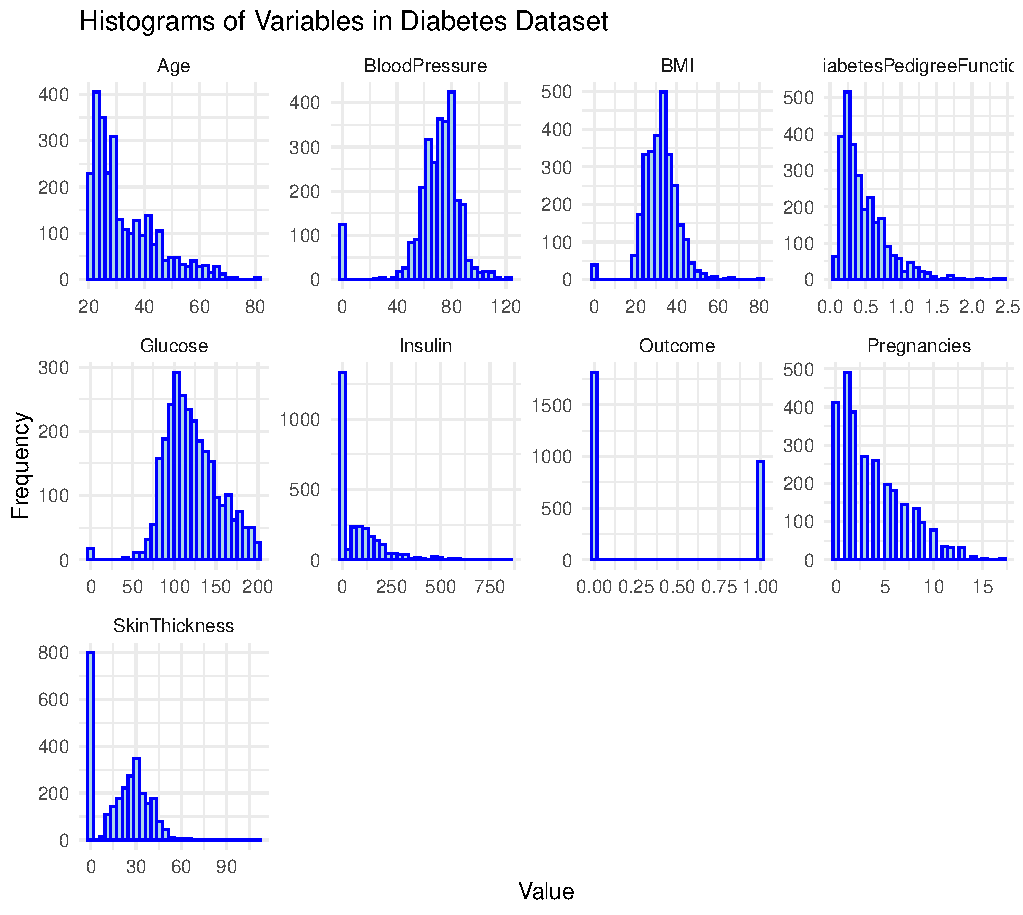
\includegraphics[width=\textwidth]{Histograms.pdf}
      \label{fig:histogram}
      \end{figure}

\section{Methods}
\label{sec:meth}
    Various methods will be used to complete the analysis necessary for this paper. I have begun by exploring basic descriptive statistics in
    the previous section in order to gain an understanding of my data set. Next, we will move on to model testing, where we will perform both 
    decision tree analysis in order to determine what predictors prove to be necessary in predicting if a patient
    will have the outcome 1 of having diabetes. 

    To begin, I will provide an explanation of what a decision tree is and why it is useful in this case. A decision tree is considered
    to be an example of supervised learning used for regression and classification. Through my analysis I will present a tree, this tree
    will begin at the top with a decision root node, which is the point where you make a decision. Following down there are subsequent sub trees
    that have other decision nodes. Finally, at the bottom of each tree you reach a leaf node, where it is the output of the decision and 
    there are no further branches off of this.  
    
    I will then begin to create my model for my decision tree by splitting the data into a test and training set. The training set will
    encompass 80 percent of the data whereas the test set will only have 20 percent. This method of splitting will help to prevent any biases that may 
    be attributed from imbalances in the distribution of critical features. After creating these two sets I will now be ready
    to build the model. This will be done by using the rpart function in R, where the method will be 'class' as this is a binary model. We will
    then see in Figure~\ref{fig:structure} the structure of the decision tree created. Looking at the leftmost path in the decision tree we 
    can see that at the top the outcome was 0 meaning that the patient did not have diabetes 35 percent of the time. Moving down to the next node, 
    we can see that 68 percent of patients with glucose level less than 128, did not have diabetes 19 percent of the time. To finish this path,
    61 percent of the time if the patient was older than 29 years old, then 8 percent of the time the patient had diabetes. The rest of the structure
    is similar but with different values and predictors.

\begin{figure}[tbp]
  \centering
  \caption{Decision Tree Structure}
  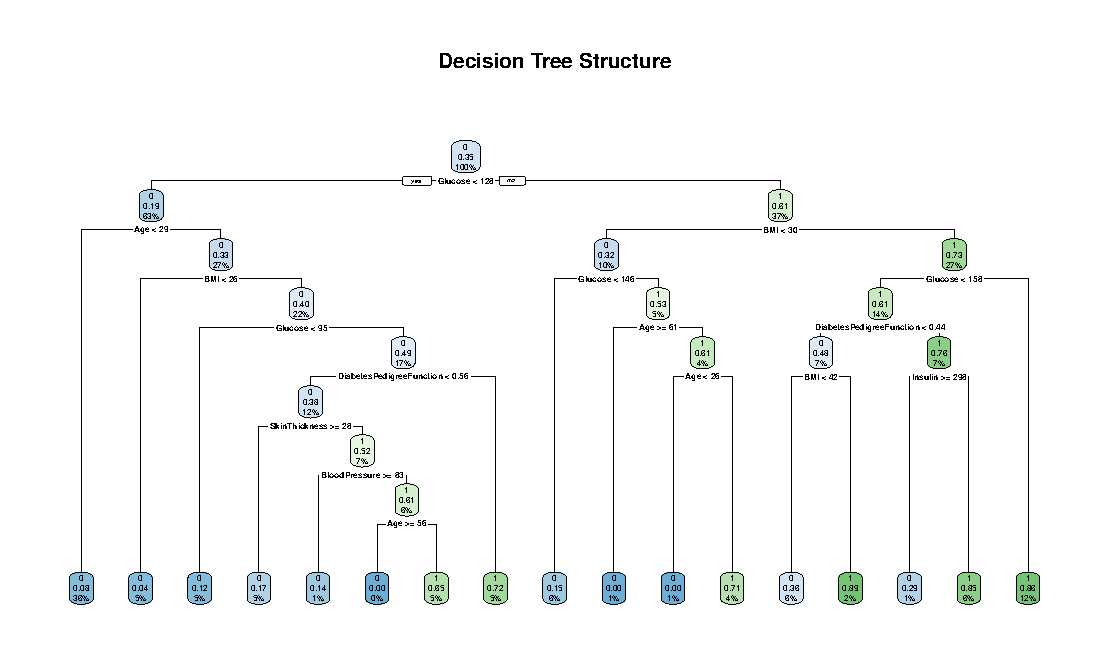
\includegraphics[width=\textwidth]{Decision Tree Structure.pdf}
  \label{fig:structure}
  \end{figure}

\section{Results}
\label{sec:resu}

After completing our methods section, we can now move on to talk about the results of our model. Based on Figure~ref{fig:importance}, we can 
see that the top three predictors are glucose, BMI, and age. The result of glucose being of the greatest importance makes complete sense with 
medical knowledge of diabetes as a patient that has high amounts of glucose in their bloodstream could have type 2 diabetes. This is known due
to glucose not being absorbed by insulin as these patients do not use insulin properly. We can see that almost all of the outcomes are explained
by glucose. The next predictor that is successful in predicting a large amount of the data is the patient's BMI. This aligns on a medical standpoint
as patients who have larger BMI values are more susceptable to getting type 2 diabetes as they are considered to be obese. Based on my results, BMI
was able to predict about half of the outcomes. The last predictor that proved to be valuable in predicting if someone has diabetes is age. This result
is somewhat medically backed but not entirely a result that I expected. Often times people that are older have diabetes due to numerous factors but it is 
not as common for younger patients.

\begin{figure}[tbp]
  \centering
  \caption{Variance Importance Plot}
  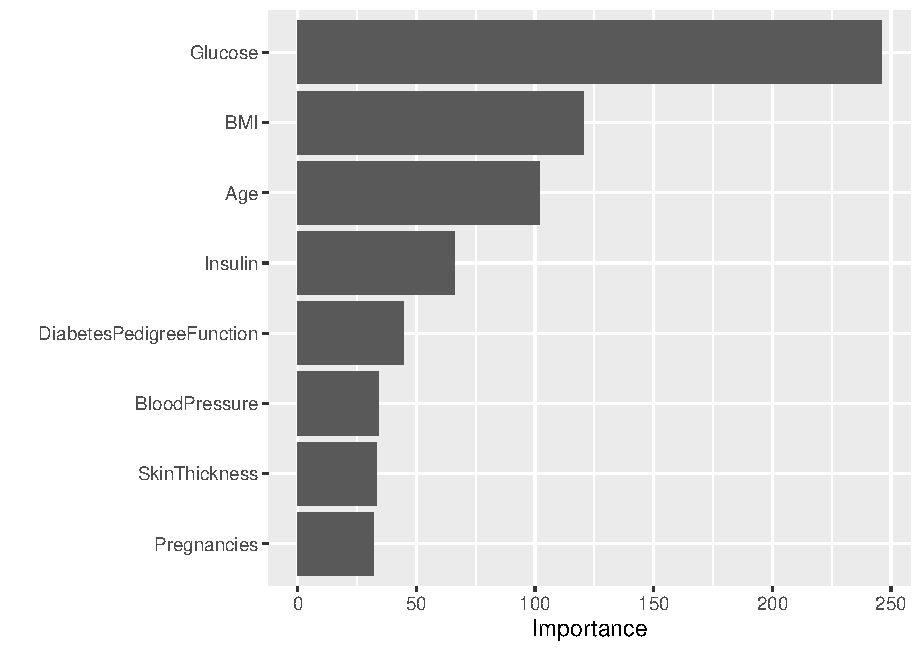
\includegraphics[width=\textwidth]{Variance Important.pdf}
  \label{fig:importance}
\end{figure}

Looking at Table~ref{tab:dtr}, we can see that the accuracy of our model is 0.82, which is high so it will be satisfactory. This tells me that we 
classify correctly 82 percent of the time out of the total instances. The next metric we will look at is precision. We were able to get to 72 percent.
This is the ratio of correctly predicted positive observations to the total predicted positives. Looking at recall, we were able to correctly identify about
74 percent of the actual positive instances. This is pretty strong and will be considered satisfactory. The final metric that we have is the F1 score, which is the
harmonic mean of precision and recall, which we were able to get a value of 0.73. This indicates a balanced performance.  

\begin{table}[ht]
  \centering
  \caption{Decision Tree Results}
  \label{tab:dtr} 
  \begin{tabular}{rrr}
    \toprule
    Metric & Value\\
    \midrule
    Accuracy & 0.82\\
    Precision & 0.72\\
    Recall & 0.74\\
    F1 Score & 0.73\\
    \bottomrule
  \end{tabular}
\end{table}

Finally we can now look at Figure~ref{fig:Heatmap}, to see the confusion matrix heatmap for our decision tree analysis. Out of the 371 patients that had an outcome
of not having diabetes, the model correctly identified 318 of them. The model only incorrectly missed a positive diagnosis 53 times. 
In terms of predicting that the patients had diabetes, the model predicted 136 patients had diabetes out of the 183 that actually did. In turn it predicted that 47 of the
patients did not have diabetes when in fact they did. This shows that the model does a pretty good job in identifying if the patient has diabetes but does an even better job
identifying when the patient does not have diabetes.  

\begin{figure}[tbp]
  \centering
  \caption{Confusion Matrix Heatmap}
  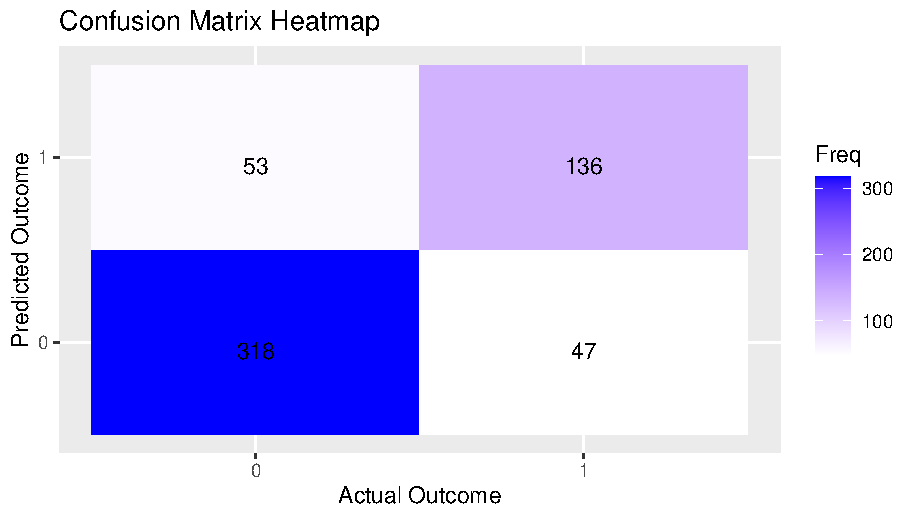
\includegraphics[width=\textwidth]{Confusion Matrix Heatmap.pdf}
  \label{fig:Heatmap}
\end{figure}

\section{Discussion}
\label{sec:disc}

Currently, this study is limited as we are set within the bounds of this data set. In future studies I can include more predictors in 
order to see if there are any other factors that could be used to predict diabetes. Moreover, I can have an even larger data set in order to 
ensure my accuracy. Other data sets may suggest that certain predictors are not helpful in predicting diabetes that my model did not pick 
up on due to the metrics of my data. 

This study can be expanded further by using other machine learning techniques to study the data. This can be used to cross-validate my results to ensure
that I am are providing the most accurate information. Other machine learning techniques could include random forest and logistic regression to give even more
understanding of the data.

As this is a paper dealing with sensitive medical data, I have many limitations in order to be ethical as well as respecting patient 
privacy. Based on the data set collected I should be able to ensure full patient privacy as names or any very unique identifiers 
are not listed with each entry. I simply have age for each entry so I do not have to worry as much for the sake of privacy as this cannot be traced
back to a particular person. In terms of our direct models I may have to disregard some assumptions as they may not fit with real world data. If something unexpected 
happens, I may have to reconsider the data set used and consider finding a new one. This will be done by a case-by-case scenario and will 
be investigated thoroughly before making any decisions.

\bibliography{refs}
\bibliographystyle{mcap}

\end{document}

